%\documentclass[a4paper]{jarticle} 
\documentclass[dvipdfmx,a4paper]{jsarticle}
\usepackage{tikz}
\usepackage{amsmath}
\usepackage{amssymb}
\topmargin = 0mm
\oddsidemargin = 5mm
\textwidth = 152mm
\textheight = 240mm


% サブセクションを 問1,問2 にする設定
\renewcommand{\thesection}{[\arabic{section}]}

% サブサブセクションを (1),(2)にする設定
\renewcommand{\thesubsection}{(\arabic{subsection})}
% (i),(ii)なら \arabic を \roman に変える。    (a),(b)なら \alph

\renewcommand{\thesubsubsection}{(\roman{subsubsection})}

% 大問2の3番目の計算式のラベルを (2.3) にする設定
% 計算式の参照には \eqref{eq:hoge} を使う
\makeatletter
  \renewcommand{\theequation}{\arabic{subsection}.\arabic{equation}}
  \@addtoreset{equation}{subsection}
\makeatother

% --------------------------------------------------------------------
\begin{document}

% タイトル
\begin{center}
\textbf{\huge{数学2D演習 第1回}}
\end{center}

%名前
\begin{flushright}
工学部電気電子工学科3年 03200489 末吉七海\\
\end{flushright}

% --------------------------------------------------------------------
% 問1
\subsection{}

%(1)
\subsubsection{}

\begin{align*}
\exp{(i\alpha + i\beta)} &= \cos{\alpha + \beta} + i\sin{\alpha + \beta} \\
&= \cos{\alpha} \cos{\beta} - \sin{\alpha} \sin{\beta} + i\cos{\alpha} \sin{\beta} + i\sin{\alpha} \cos{\beta} \\
&=(\cos{\alpha} + i\sin{\alpha})(\cos{\beta} + i\sin{\beta}) \\
&=\exp{(i\alpha)} \exp{(i\beta)}
\end{align*}

より示された。

%(2)
\subsubsection{}

(1)において、$\alpha = \theta$、$\beta = \theta$とおくと、

\begin{align*}
\bigl(\exp{(i\theta)}\bigr)^2 &= \exp{(2i\theta)}
\end{align*}

Eularの公式を用いて、

\begin{align*}
(\cos{\theta} + i\sin{\theta})^2 &= \cos{2\theta} + i\sin{2\theta} \\
\cos^{2}\theta - \sin^{2}\theta + i2\sin{\theta} \cos{\theta} &= \cos{2\theta} + i\sin{2\theta}
\end{align*}

上式の実部と虚部を比較して、

\begin{align*}
\cos{2\theta} &= \cos^{2}\theta - \sin^{2}\theta\\
\sin{2\theta} &= 2\sin{\theta} \cos{\theta}
\end{align*}

以上より、2倍角の公式が導かれた。\\
\\

(1)において、$\alpha = 2\theta$、$\beta = \theta$とおくと、

\begin{align*}
\exp{(i\theta)} \exp{(2i\theta)} &= \exp{(3i\theta)}
\end{align*}

Eularの公式を用いて、

\begin{align*}
(\cos{\theta} + i\sin{\theta})(\cos{2\theta} +i\sin{2\theta}) &= \cos{3\theta} + i\sin{3\theta} \\
(\cos{\theta} + i\sin{\theta})(\cos^{2}\theta - \sin^{2}\theta + i2\cos{\theta} \sin{\theta})&= \cos{3\theta} + i\sin{3\theta}\\
\cos^{3}\theta - 3\cos{\theta} \sin^{2}\theta +i3\cos^{2}\theta \sin{\theta} - i\sin^{3}\theta &= cos3\theta + isin3\theta\\
4\cos{^3}\theta - 3\cos{\theta} - i4\sin^{3}\theta + i3\sin{\theta} &= \cos{3\theta} + i\sin{3\theta}
\end{align*}

上式の実部と虚部を比較して、

\begin{align*}
\cos{3\theta} &= 4\cos^{3}\theta - 3\cos{\theta}\\
\sin{3\theta} &= 3\sin{\theta} - 4\sin^{3}\theta
\end{align*}

以上より3倍角の公式が導かれた。\\

%(3)
\subsubsection{}

Eularの公式を用いて、

\begin{align*}
z &= \exp{(3+ 1i)}\\
&= \exp{(3)}\exp{(1i)} \\
&= \exp{(3)} (\cos{1} + i\sin{1})\\
&= \exp{(3)}\cos{1} + i\exp{(3)}\sin{1}
\end{align*}

点z(exp(3)cos1 + iexp(3)sin1)を複素平面上に図示すると、\\

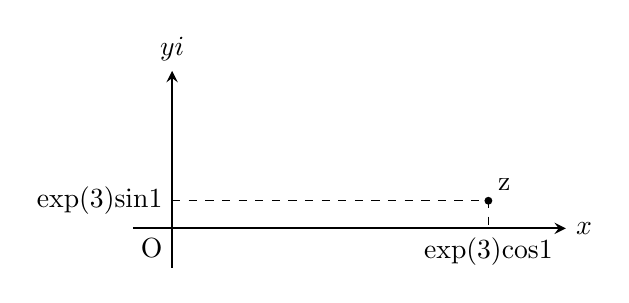
\begin{tikzpicture}
 \coordinate[label=below left:O] (O) at (0,0); %原点O
 \coordinate (XS) at (-0.5,0); %x軸最小
 \coordinate (XL) at (5,0); %x軸最大
 \coordinate (YS) at (0,-0.5); %y軸最小
 \coordinate (YL) at (0,2); %y軸最大
 \draw[thick,->,>=stealth] (XS)--(XL) node[right] {$x$}; %x軸
 \draw[thick,->,>=stealth] (YS)--(YL) node[above] {$yi$}; %y軸
 \coordinate[label=above right:z] (z) at ({exp(3)*cos(1)/5}, {exp(3)*sin(1)}); %点z
 \fill (z) circle (0.05); %zの塗りつぶし
 \draw[dashed] (0,{exp(3)*sin(1)})node[left]{exp(3)sin1}--(z)--({exp(3)*cos(1)/5},0)node[below]{exp(3)cos1}; %zの座標を示す波線
\end{tikzpicture}

%(4)
\subsubsection{}

\begin{flushleft}
(4-1)
\end{flushleft}
rは点zの原点からの距離を表す。\\
$\theta$は半直線Ozとx軸性方向とのなす角を表す。\\


\begin{flushleft}
(4-2)
\end{flushleft}

$0 < \theta < 2\pi$に注意して、

\begin{align*}
1 + i &= \sqrt{2}(\frac{1}{\sqrt{2}} + i\frac{1}{\sqrt{2}})\\
&= \sqrt{2}(\cos{\frac{\pi}{4}}+ i\sin{\frac{\pi}{4}})\\
&= \sqrt{2}\exp{i\frac{\pi}{4}}
\end{align*}
\\
\\
\\

\begin{flushleft}
(4-3)
\end{flushleft}
 
 \begin{align*}
 z_1z_2 &= r_1r_2\exp{\bigl(i(\theta_1+\theta_2)\bigr)}\\
 \frac{z_1}{z_2} &= \frac{r_1}{r_2}\exp{\bigl(i(\theta_1-\theta_2)\bigr)}
 \end{align*}
 
 より、$z_1z_2$の絶対値は$r_1r_2$、偏角は$\theta_1+\theta_2$、また$\frac{z_1}{z_2}$の絶対値は$\frac{r_1}{r_2}$、偏角は$\theta_1-\theta_2$である。
 
 %(5)
 \subsubsection{}
 
 $A = r_1\exp{(i\theta_1)}$、$B = r_2\exp{(i\theta_2)}$とおくと、
 
  \begin{align*}
  \exp{(A)}\exp{(B)} &= (\sum_{n=0}^{\infty}\frac{1}{n!}A^n)(\sum_{n=0}^{\infty}\frac{1}{n!}B^n)\\
  &= \Bigl(\sum_{n=0}^{\infty}\frac{1}{n!}\bigl(r_1\exp{(i\theta_1)}\bigr)^n\Bigr)\Bigl(\sum_{n=0}^{\infty}\frac{1}{n!}\bigl(r_2\exp{(i\theta_2)}\bigr)^n\Bigr)\\
  &= \Bigl(1 + \frac{r_1\exp{(i\theta_1)}}{1!} + \frac{\bigl(r_1\exp{(i\theta_1)}\bigr)^2}{2!} + \cdots + \frac{\bigl(r_1\exp{(i\theta_1)}\bigr)^n}{n!} + \cdots\Bigr)\\
  &\qquad\Bigl(1 + \frac{r_2\exp{(i\theta_2)}}{1!} + \frac{\bigl(r_2\exp{(i\theta_2)}\bigr)^2}{2!} + \cdots + \frac{\bigl(r_2\exp{(i\theta_2)}\bigr)^n}{n!} + \cdots\Bigr)\\
  &= 1 + \frac{r_1exp{(i\theta_1)} + r_2\exp{(i\theta_2)}}{1!} + \frac{r_1^2\exp{(2i\theta_1)} + 2r_1r_2\exp{\bigl(i(\theta_1+\theta_2)\bigr)} + r_2^2\exp{2i\theta_2)}}{2!} + \cdots \\
  &\qquad + \frac{\sum_{m=1}^{n}r_1^mr_2^{(n-m)}\exp{\Bigl(i\bigl(m\theta_1 + (n-m)\theta_2\bigr)\Bigr)}\frac{n!}{m!(n-m)!}}{n!} + \cdots\\
  &= \sum_{m=0}^{\infty}\frac{\bigl(r_1\exp{(i\theta_1)} + r_2\exp{(i\theta_2)}\bigr)^m}{m!}\\
  &= \sum_{n=0}^{\infty}\frac{1}{n!}(A+B)^n\\
  &= \exp{(A+B)}
 \end{align*}
 
 以上より示された。\\
 
% --------------------------------------------------------------------
% 問2
\subsection{}

\subsubsection{}

三角形$\alpha\beta\gamma$が正三角形と必要十分条件は、角$\gamma = \frac{1}{3}\pi$かつ $|\alpha-\gamma| = |\beta-\gamma|$なので、\\
$\gamma$に関して$\alpha$と$\beta$の左右は問わないことに注意すると、

\begin{align*}
\alpha-\gamma &= (\beta-\gamma)\exp{(i\pm\frac{1}{3}\pi)}\\
&= (\beta-\gamma)(\cos{\pm\frac{1}{3}\pi} + i\sin{\pm\frac{1}{3}\pi})\\
&= (\beta-\gamma)(\frac{1}{2} \pm \frac{\sqrt{3}}{2}i)
\end{align*}

以上より、
\begin{align*}
\frac{\alpha-\gamma}{\beta-\gamma} = \frac{1\pm\sqrt{3}i}{2}
\end{align*}

\subsubsection{}

(1)より、
\begin{align*}
\alpha-\gamma &= (\beta-\gamma)(\frac{1}{2} \pm \frac{\sqrt{3}}{2}i)\\
2(\alpha\gamma) &= (\beta-\gamma)(1\pm\sqrt{3}i)\\
2\alpha - \beta - \gamma &= \sqrt{3}i(\beta - \gamma)\\
\bigl(2\alpha - \beta - \gamma\bigr)^2 &= \bigl(\sqrt{3}i(\beta - \gamma)\bigr)^2\\
4\alpha^2 + \beta^2 + \gamma^2 - 4\alpha\beta + 2\beta\gamma - 4\gamma\alpha &= -3\beta^2 +6\beta\gamma -3\gamma^2\\
4\alpha^2 + 4\beta^2 + 4\gamma^2 - 4\alpha\beta - 4\beta\gamma - 4\gamma\alpha &= 0\\
\alpha^2 + \beta^2 + \gamma^2 - \alpha\beta -\beta\gamma -\gamma\alpha &= 0
\end{align*}

以上より示された。


%-----------------------------------
%問3
\subsection{}

\subsubsection{}
\begin{align*}
(与式) &= \sum_{n=0}^{\infty}\frac{1}{n!}z^n\\
\therefore\quad
a_n &= \frac{1}{n!}
\end{align*}

収束半径rは
\begin{align*}
r &= \lim_{n \to \infty}\Bigl|\frac{a_n}{a_{n+1}}\Bigr|\\
&= \lim_{n \to \infty}\biggl|\frac{\frac{1}{n!}}{\frac{1}{(n+1)!}}\biggr|\\
&= \lim_{n \to \infty}\Bigl|\frac{(n+1)!}{n!}\Bigr|\\
&= \lim_{n\to \infty}|n+1|\\
&= \infty
\end{align*}

\subsubsection{}
\begin{align*}
(与式) &= \sum_{n=0}^{\infty}\frac{(-1)^{n-1}}{n}z^n\\
\therefore\quad
a_n &= \frac{(-1)^{n-1}}{n}
\end{align*}

収束半径rは
\begin{align*}
r &= \lim_{n \to \infty}\Bigl|\frac{a_n}{a_{n+1}}\Bigr|\\
&= \lim_{n \to \infty}\biggl|\frac{\frac{(-1)^{n-1}}{n}}{\frac{(-1)^{n}}{n+1}}\biggr|\\
&= \lim_{n \to \infty}\Bigl|-\frac{n+1}{n}\Bigr|\\
&= 1
\end{align*}

\subsubsection{}
\begin{align*}
(与式) &= \sum_{n=0}^{\infty}\frac{\alpha(\alpha-1)\cdots(\alpha-n)}{n!}z^n\\
\therefore\quad
a_n &= \frac{\alpha(\alpha-1)\cdots(\alpha-n)}{n!}
\end{align*}

収束半径rは
\begin{align*}
r &= \lim_{n \to \infty}\Bigl|\frac{a_n}{a_{n+1}}\Bigr|\\
&= \lim_{n \to \infty}\Biggl|\frac{\frac{\alpha(\alpha-1)\cdots(\alpha-n)}{n!}}{\frac{\alpha(\alpha-1)\cdots(\alpha-n)(\alpha-n-1)}{(n+1)!}}\Biggr|\\
&= \lim_{n \to \infty}\Bigl|\frac{n+1}{\alpha-n-1}\Bigr|\\
&= 1
\end{align*}

\end{document}